\label{chap:impl}

\subsection{Placing Algorithm}
 
The placing algorithm is at its core a genetic algorithm \cite{chambers2010practical}, which uses
a specified set of heuristic functions to compute the fitness of individuals.
An individual is represented by the configuration of the graph at a certain, i.e.
the location of each node.

The idea behind the algorithm is to try and place the graph in a natural way, similar
to how a human would do it by hand. Because every person prefers a different type of 
layout or arrangement, the placing algorithm uses constraints specified by the user
to verify if the graph has been properly placed.

The algorithm starts by creating a generation composed of individuals which have 
been randomly placed on the canvas. It then proceeds to check how good each 
individual is by computing its fitness. This will yield a subset of layouts which
are the closest aproximation of what the user desired. At this point, for each 
part of individual (i.e. a node) it further computes a score, depending on the
number of connections and where it has been placed. Then, two individuals are 
picked and a recombination will be performed. Four new individuals shall be obtained:
one which has the best positions from both parents, one which has the worst positions
from each parent and the last two which have the best from one parent and the 
worst from the other, and vice-versa.

At the end of recombination, a new generation will have been obtained. This selective 
evolution process \cite{goldberg2006genetic} will continue until either stability has been achieved (there is an
individual with the best fitness which appears constantly in every generation) or, for 
performance reasons, a certain number of generations has passed. The individual with 
the best fitness shall represent the final layout.

\begin{figure*}[ht] \centering
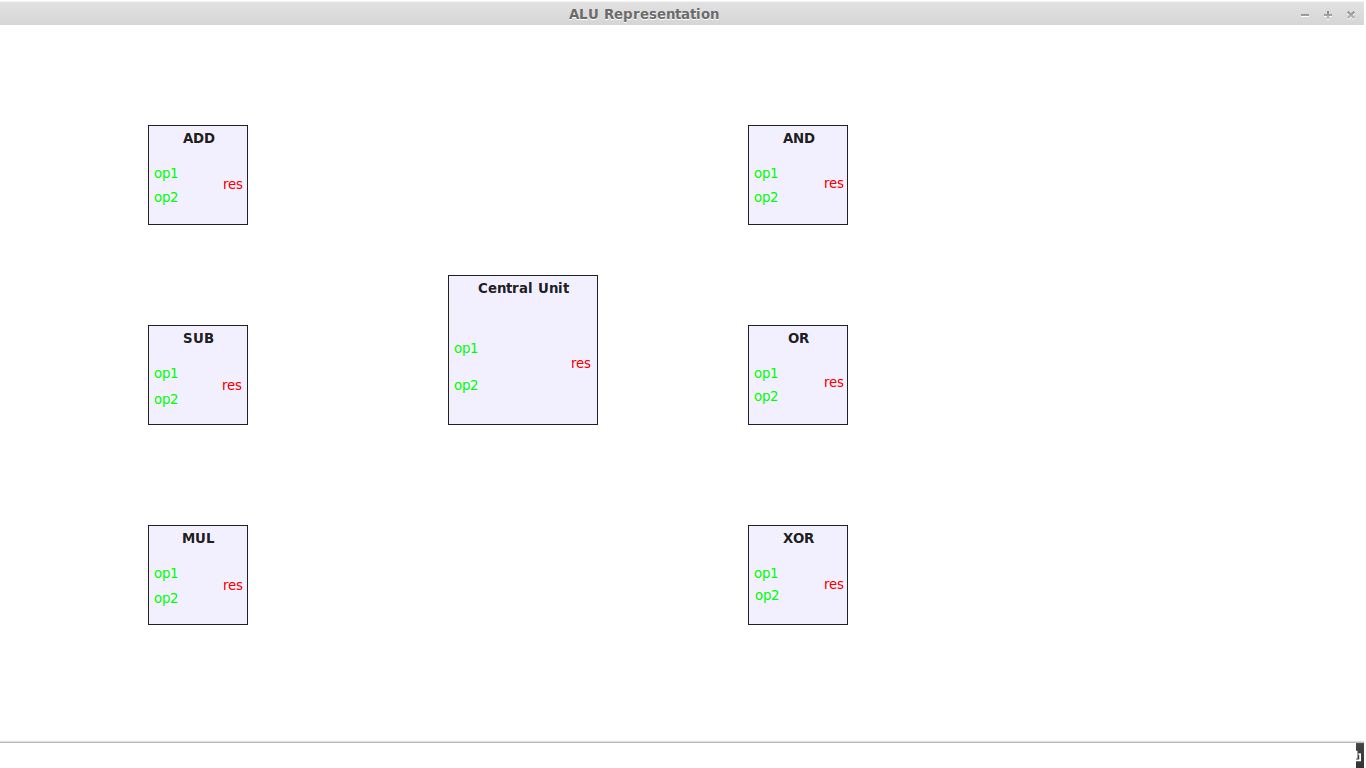
\includegraphics[width=0.8\textwidth]{src/placingLogic.png}
\caption{ALU unit components placing: logical units split from arithmetic units.} \end{figure*}

\subsection{Routing Algorithm}

The routing algorithm is based on the orthogonal edge routing. This method ensures 
that all the edges which compose a connection path are orthogonal. Also, another 
imposed restriction is that, when possible, no path should cross another path to 
avoid creating confusing intersection points.

The algorithm mixes a shortest path approach with an original take on avoiding obstacles.
At first, in order to route a path, the shortest path between the two components that have 
to be connected is computed, ensuring that it avoids obstacles. Then, all redundant points 
are eliminated (a redundant point is any point C which is on a valid segment [AB]). After 
this step, the path is "orthogonalized", meaning that all edges which are not orthogonal are 
broken into smaller, orthogonal edges. Should any of these new segments intersect an obstacle,
that segment shall be treated as a separate route and re-computed so that it no longer 
intersects the obstacle.

Should the computed path intersect any other already existing path, a new one shall be 
computed. It will no longer be the shortest, but it will trade area covered by the drawing 
for clarity and better understanding of the graph.

\begin{figure}[ht] \centering
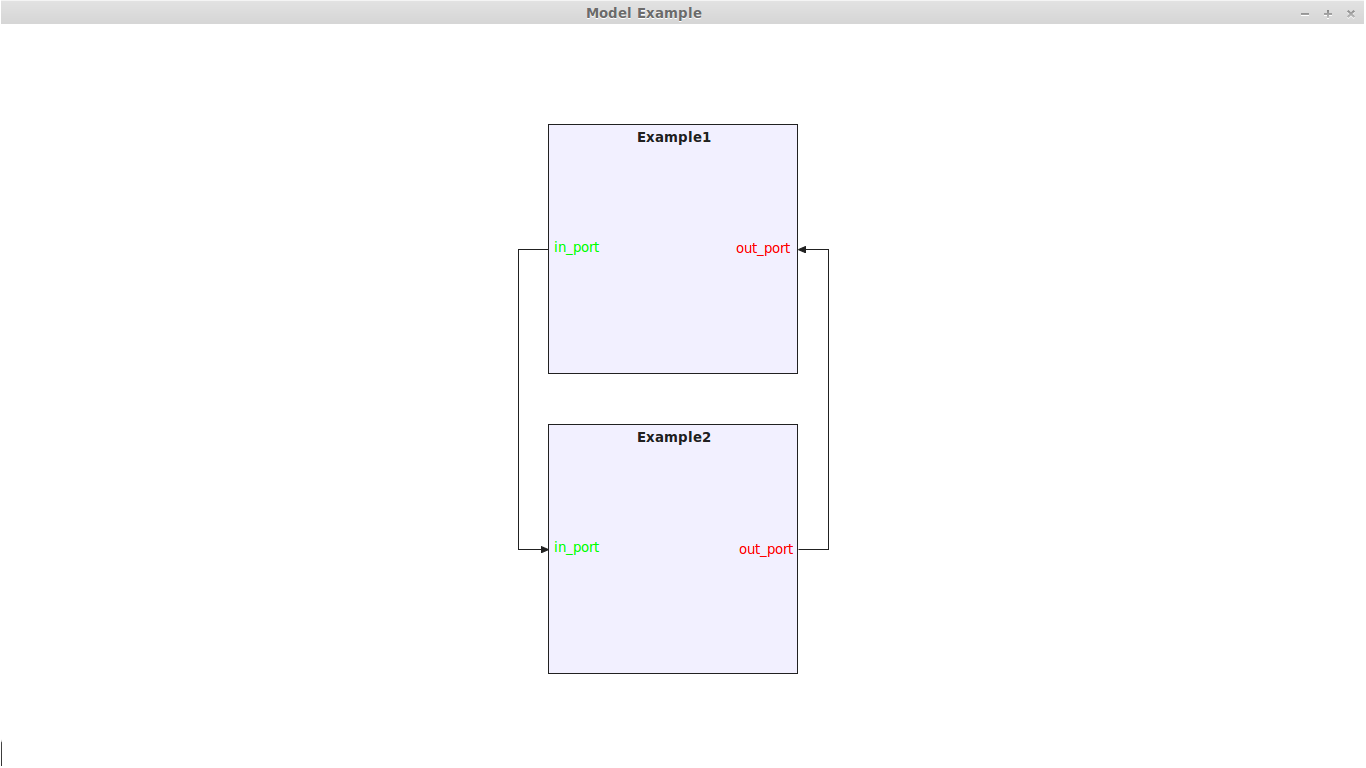
\includegraphics[width=0.5\textwidth]{src/modelExample.png}
\caption{The general look of nodes and routes in the model. Input ports are highlited green; output ports are highlighted red; arrow decorations are placed 
at the end of a route to show its direction.} \end{figure}
